
Nowadays, it is not uncommon for many types of users
--- from proficient data scientists to enthusiasts without formal
training, from finance to physics --- to dive into overwhelming
data sets looking for any relevant pattern they can find. This data
may consist of files that have not yet been ingested into a
database system. The researcher must curate
these files, understand and sieve their content, and 
extract information. This data-intensive way of doing science is considered
a new paradigm of scientific exploration, the fourth after the experimental, theoretical, and computer-simulation paradigms~\cite{bell2009beyond,hey2009the}.

The activity of data exploration is usually referred to as \gls{KDD}
because ``knowledge'' is the product of this process
\parencite{Piatetsky-Shapiro1991,Fayyad1996a}.
\emph{Data Mining} is sometimes used as a synonym or as an integral
part, as shown in figure~\ref{fig:kdd} \cite{Fayyad1996a,Reinartz1999}.
The latter interpretation is preferred for this work. 

\begin{figure}[htbp]
    \centering
    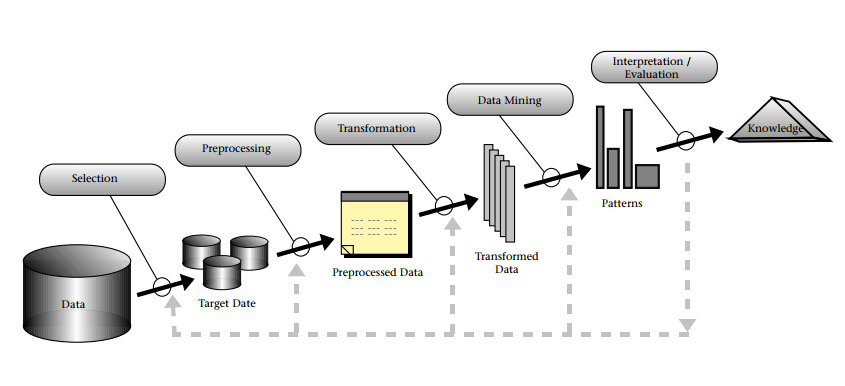
\includegraphics[width=\linewidth]{images/1_introduction/kdd.jpg}
    \caption{\glsfmtfull{KDD}.}
    \label{fig:kdd}
\end{figure}

The \gls{CRISPDM}~\cite{Shearer2000} proposes a model for the data
mining step, composed of six phases, shown in figure~\ref{fig:crispdm}:

\begin{description}
    \item[Business Understanding] Definition of the requirements and objectives of a data mining project
        from the business (or domain) perspective.
    \item[Data Understanding] Familiarization with the data collection. Domain knowledge
        is needed to understand the data, but the original project can be refined as the data is best understood.
    \item[Data Preparation] Attribute selection, cleaning, imputation, \ldots are applied over the raw data.
    \item[Modeling] Various modeling techniques are implemented, calibrated and assessed. Different models may require different data preparation ---
    for instance, cleaning, imputation, or normalization.
    \item[Evaluation] The proposed models need to be thoroughly reviewed to make sure they meet the required quality and that they achieve the stated
    objectives.
    \item[Deployment] The new knowledge has to be useful and actionable.
    Depending on the original objectives, the model can be integrated 
    or transformed into an automatic system; or ``simply'' summarized into a report.
\end{description}

\begin{figure}[htb]
    \centering
    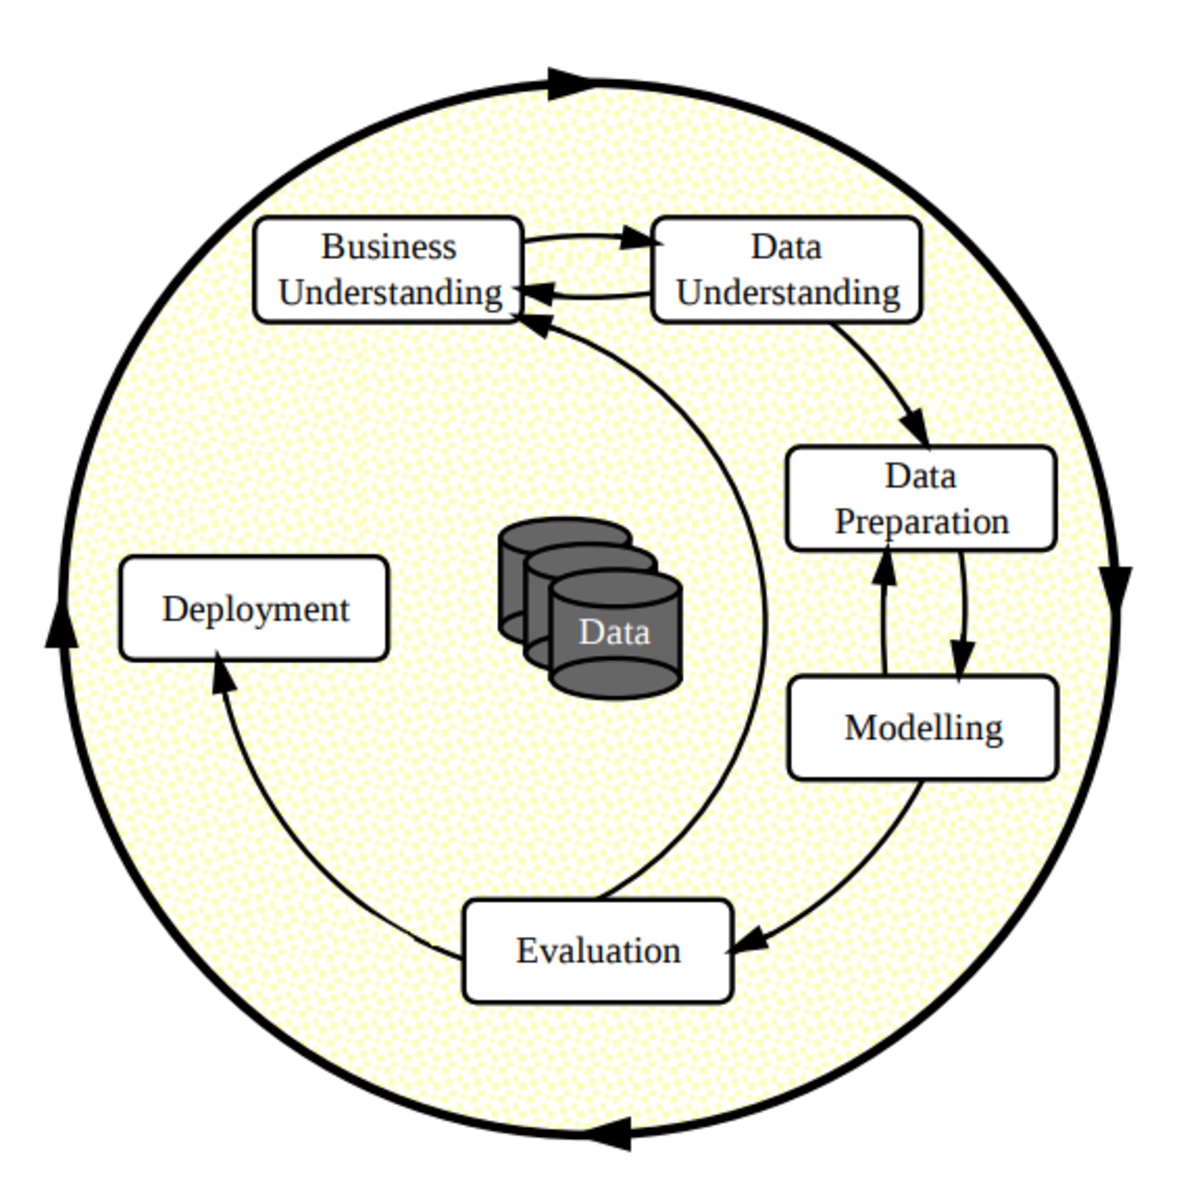
\includegraphics[width=0.8\linewidth]{images/1_introduction/crisp-dm.pdf}
    \caption{\glsfmtfull{CRISPDM}.}
    \label{fig:crispdm}
\end{figure}

In this thesis, we focus on the \textbf{Data Understanding} phase, where the user interactively
explores the data, gaining insight, and generating hypotheses during the process.

When starting the initial analysis, the data may be in a \emph{raw} format: unprocessed files not optimized for access. Even worse, their schema may be inconsistent or poorly documented, and they may originate from different sources. These factors combined difficult the task of the data scientist:

\begin{itemize}
    \item Ingestion into a ``proper'' database introduces latency. Since the data is not well
        understood, any early design decision will soon become obsolete~\cite{Kersten2011}.
        Techniques for \emph{in-situ} exploration try to overcome this difficulty
        by allowing direct examination of the data files performantly~\cite{Idreos2011}.
    \item The data may be split into multiple files~\cite{Baud2012}, and these files may not
        follow the same schema~\cite{Alawini2014}. Data profiling and schema-matching tools
        can be helpful for this type of problem.
\end{itemize}

Unfortunately, \emph{in-situ} techniques leave out schema-matching, while the existing
data profiling approaches require either relational data from discrete domains or they are restricted to matching based on a single attribute. This motivates our
research.

\section{Objectives}
\label{sec:main_objective}

Given the problem stated above, the main objective of this
thesis is \emph{to assist users during the exploration of unprocessed,
numerical, raw data distributed across multiple files,
based solely on its intrinsic distribution}. For this
object, we need to:

\begin{enumerate}
    \item Find and evaluate existing techniques that could help users to
    understand the data files \emph{in-situ}.
    \item Identify gaps in the coverage of the existing techniques.
    \item To reduce these gaps, design algorithms tailored to numerical and uncertain data.
    \item Evaluate their performance.
\end{enumerate}
\label{enum:objectives}

\section{Structure of this document}

First, we described the methodology followed for this thesis in chapter~\ref{chapter:methodology}.
Chapter~\ref{chapter:literature_review} contains a systematic literature mapping
of the \emph{in-situ} processing of scientific data.
Then, chapter~\ref{chapter:diverse} identifies gaps in the literature regarding
the exploration of diverse numerical datasets and summarizes some initial prototypes
that remain open for further research.
Chapter~\ref{chapter:presq} proposes an algorithm suitable for schema matching
tailored to scientific data. Chapter~\ref{chapter:som} outlines a statistical
test based on \glspl{SOM}, which can bridge the gap between schema matching and
\emph{in-situ} access.
Chapter~\ref{chapter:discussion} discusses our contributions
and analyses the threats to the validity of the present thesis.
Finally, chapter~\ref{chapter:conclusions} summarizes our findings and contributions and proposes potential future lines of work.
